\section{(Continuous) Uniform Distribution ( $U(a, b)$ )}

\begin{table}[H]
    \hfill
    \begin{minipage}{0.45\linewidth}
        \begin{figure}[H]
            \centering
            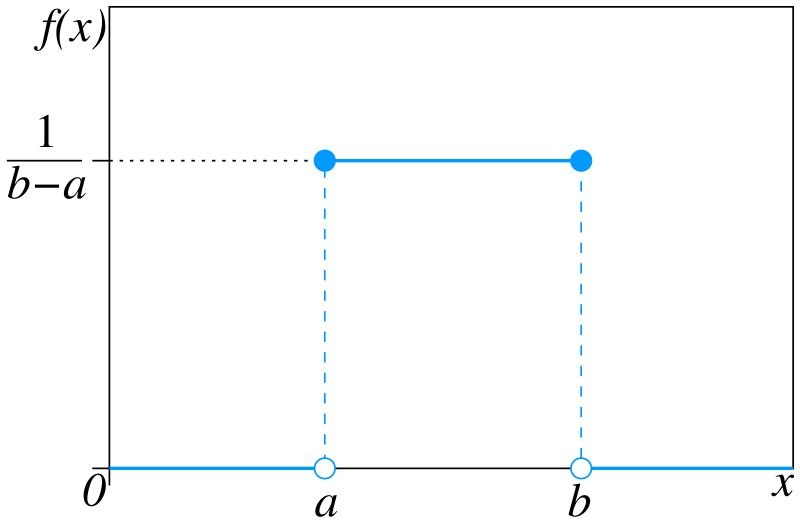
\includegraphics[
                width=\linewidth,
                height=5cm,
                keepaspectratio,
            ]{images/distributions/Uniform_Distribution_PDF_SVG.svg}
            \caption{Uniform Distribution: PDF \cite{wiki/Continuous_uniform_distribution}}
        \end{figure}
    \end{minipage}
    \hfill
    \begin{minipage}{0.45\linewidth}
        \begin{figure}[H]
            \centering
            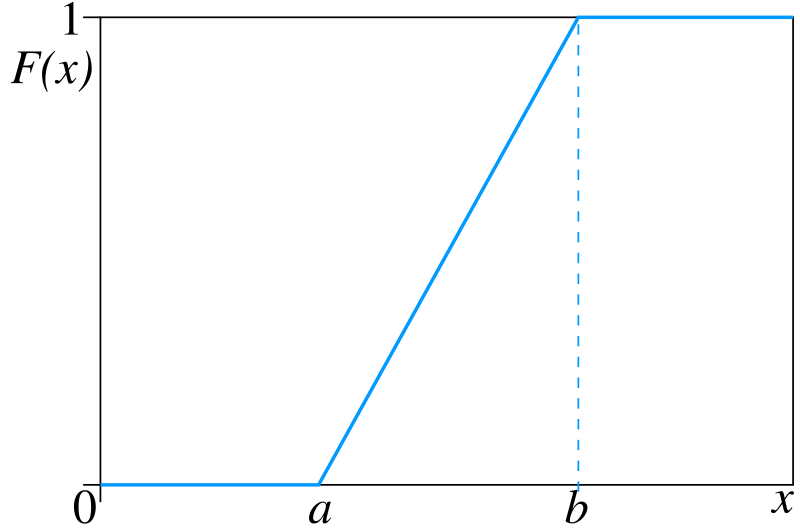
\includegraphics[
                width=\linewidth,
                height=5cm,
                keepaspectratio,
            ]{images/distributions/Uniform_Distribution_CDF_SVG.svg}
            \caption{Uniform Distribution: CDF \cite{wiki/Continuous_uniform_distribution}}
        \end{figure}
    \end{minipage}
    \hfill
\end{table}

\subsection{PDF}

\begin{enumerate}
    \item[] $f_{a,b}(x) = \dfrac {1}{b-a}, \hspace{1cm} x \in [a, b]$
    \hfill \cite{statistics/book/Statistics-for-Data-Scientists/Maurits-Kaptein}

    \item If the random measurement error would be described by a uniform PDF, being close to or far away form zero would be equally likely.
    However, the uniform PDF has a finite domain, which means that the density is positive on an interval, say $[a, b]$, with $a < b$ and $a, b \in \mbbR$, but zero everywhere else.
    \hfill \cite{statistics/book/Statistics-for-Data-Scientists/Maurits-Kaptein}
\end{enumerate}



\subsection{Summary}

\begin{enumerate}
    \item \textbf{Notation}:
    ${\displaystyle {\mathcal {U}}_{[a,b]}}$
    \hfill \cite{wiki/Continuous_uniform_distribution}

    \item \textbf{Parameters}:
    ${\displaystyle -\infty <a<b<\infty }$
    \hfill \cite{wiki/Continuous_uniform_distribution}

    \item \textbf{Support}: $[a, b]$
    \hfill \cite{wiki/Continuous_uniform_distribution}

    \item \textbf{PDF}:
    $
        {\displaystyle {\begin{cases}{\dfrac {1}{b-a}}&{\text{for }}x\in [a,b]\\0&{\text{otherwise}}\end{cases}}}
    $
    \hfill \cite{wiki/Continuous_uniform_distribution, statistics/book/Statistics-for-Data-Scientists/Maurits-Kaptein}

    \item \textbf{CDF}:
    $
        {\displaystyle {\begin{cases}0&{\text{for }}x<a\\{\dfrac {x-a}{b-a}}&{\text{for }}x\in [a,b]\\1&{\text{for }}x>b\end{cases}}}
    $
    \hfill \cite{wiki/Continuous_uniform_distribution}

    \item \textbf{Mean}:
    $
        {\displaystyle {\dfrac {1}{2}}(a+b)}
    $
    \hfill \cite{wiki/Continuous_uniform_distribution}

    \item \textbf{Median}:
    $
        {\displaystyle {\dfrac {1}{2}}(a+b)}
    $
    \hfill \cite{wiki/Continuous_uniform_distribution}

    \item \textbf{Mode}:
    any value in $ {\displaystyle (a,b)} $
    \hfill \cite{wiki/Continuous_uniform_distribution}

    \item \textbf{Variance}:
    $
        {\displaystyle {\dfrac {1}{12}}(b-a)^{2}}
    $
    \hfill \cite{wiki/Continuous_uniform_distribution}

    \item \textbf{Median absolute deviation (MAD)}:
    $
        {\displaystyle {\dfrac {1}{4}}(b-a)}
    $
    \hfill \cite{wiki/Continuous_uniform_distribution}

    \item \textbf{Skewness}:
    $0$
    \hfill \cite{wiki/Continuous_uniform_distribution}

    \item \textbf{Excess kurtosis}:
    $ -\dfrac{6}{5}$
    \hfill \cite{wiki/Continuous_uniform_distribution}

    \item \textbf{Entropy}: $ {\displaystyle \log(b-a)} $
    \hfill \cite{wiki/Continuous_uniform_distribution}

    \item \textbf{Moment-generating function (MGF)}:
    $
        {\displaystyle {\begin{cases}{\dfrac {\mathrm {e} ^{tb}-\mathrm {e} ^{ta}}{t(b-a)}}&{\text{for }}t\neq 0\\1&{\text{for }}t=0\end{cases}}}
    $
    \hfill \cite{wiki/Continuous_uniform_distribution}

    \item \textbf{Characteristic function (CF)}:
    $
        {\displaystyle {\begin{cases}{\dfrac {\mathrm {e} ^{\mathrm {i} tb}-\mathrm {e} ^{\mathrm {i} ta}}{\mathrm {i} t(b-a)}}&{\text{for }}t\neq 0\\1&{\text{for }}t=0\end{cases}}}
    $
    \hfill \cite{wiki/Continuous_uniform_distribution}

\end{enumerate}







